\documentclass[sigconf,anonymous]{acmart}

% Add the review option above to display reviewer line numbers.
% Keep anonymous for the double-blind submission.
% This is a writing template: replace all Writing guide paragraphs.
\newcommand{\writingguide}[1]{\par\noindent\textit{Writing guide: #1}\par}

% Anonymous FPGA '27 draft: retain ACM's reference block and conference footer.
% Do not claim a publication license or use unassigned DOI/ISBN placeholders.
% Replace the rights and publication metadata with ACM's eRights values
% when preparing the accepted paper.
\setcopyright{none}
\settopmatter{printacmref=true,printccs=true,printfolios=true}
\acmDOI{}
\acmISBN{}
% Public conference information for the draft header, from the FPGA'27 CFP.
% Replace publication metadata with ACM's supplied values after acceptance.
\acmConference[FPGA '27]{35th ACM/SIGDA International Symposium on Field-Programmable Gate Arrays}{March 14--16, 2027}{California, USA}
\acmYear{2027}
\copyrightyear{2027}

\title[FHEStore: Bridging Persistent Data and FHE Accelerators]{FHEStore: Bridging Persistent Data and FHE Accelerators with FPGA-Based Computational Storage}

% Author and affiliation fields are intentionally omitted during review.
% For the accepted version, remove anonymous and add real author metadata.
% Add the publication metadata supplied by ACM only after acceptance.
% \author{Author name}
% \affiliation{\institution{Institution}\city{City}\country{Country}}
% \email{author@example.org}
% \acmSubmissionID{ID supplied by the submission system}

\begin{document}

\begin{abstract}
Fully homomorphic encryption (FHE) accelerators act as ciphertext consumers, substantially reducing the cost of homomorphic computation. However, producing their inputs from persistent data introduces additional overhead. Conventionally, the host serves as the input producer, using CPU and memory resources for data access, preprocessing, encryption, and buffering. Ciphertext expansion further increases buffering and data-movement costs.

We present FHEStore, an FPGA-based computational storage system that bridges persistent data and FHE accelerators through storage-side ciphertext production. FHEStore combines storage-side data access with an FPGA streaming datapath to integrate lightweight preprocessing, encoding, and Fast Fully Homomorphic Encryption over the Torus (TFHE) encryption. A shared operator stream switch connects device-local input buffers to the processing operators and collects their ciphertext output for host delivery.

We prototype FHEStore on an FPGA-enabled computational storage device and integrate it with a remote homomorphic processing unit (HPU). For TFHE encryption of unsigned 8-bit data with a batch size of 4~KiB, the FPGA encryption engine achieves a $5.33\times$ speedup over host CPU-based encryption. In the evaluated end-to-end input production workflow, FHEStore achieves a $3.26\times$ speedup over the host-based baseline. We also demonstrate homomorphic computation on the remote HPU using FHEStore-generated ciphertexts.
\end{abstract}

% Draft CCS selections. Generate the matching CCSXML through ACM's CCS
% tool before preparing the submission metadata.
\ccsdesc[500]{Hardware~Reconfigurable logic and FPGAs}
\ccsdesc[300]{Information systems~Storage architectures}
\ccsdesc[300]{Security and privacy~Cryptography}
\keywords{Fully homomorphic encryption, TFHE, FPGA, high-level synthesis, computational storage, streaming dataflow}

\maketitle

\section{Introduction}
\label{sec:introduction}
Fully homomorphic encryption (FHE) enables a data owner to outsource computation over encrypted data without revealing the plaintext to the evaluator. For applications backed by persistent data, an input producer accesses application data and generates the ciphertexts that an FHE accelerator consumes. This producer connects persistent application data with encrypted computation, and its data access, preprocessing, and encryption costs remain part of the application workflow.

Dedicated hardware research addresses encryption cost through specialized encryption architectures~\cite{mert2020bfv,lee2023ckks,feryputri2025lwe,syafalni2026multicore}. Specialized arithmetic and parallel datapaths make encryption a practical acceleration target across FHE schemes. Translating encryption acceleration into an application benefit also requires connecting the operator to data preparation and ciphertext transfer. The cost of those surrounding stages depends on where encryption is placed and how data are handed between stages.

Research on memory-aware FHE accelerators complements arithmetic acceleration by optimizing data reuse, memory access, and traffic during homomorphic computation~\cite{xu2026hera,zhou2023fhemem,vanbeirendonck2023fpt,kim2022bts,kim2022ark}. This work establishes the expanded ciphertext representation and large cryptographic working sets, including evaluation keys, as architectural concerns alongside arithmetic. The resulting data layouts, memory organizations, and streaming schedules improve the execution of homomorphic programs. Their optimization boundary centers on the working set consumed by encrypted computation. Application workflows additionally need to generate input ciphertexts from persistent data; organizing this production path is a complementary systems problem.

Client-side systems further combine cryptographic acceleration with encoding, memory organization, streaming, buffering, or client--server communication~\cite{krieger2024aloha,yune2025abcfhe,vanderhagen2022choco,gupta2024memfhe}. Their client-side processing paths connect cryptographic stages to memory or communication interfaces. For applications whose inputs reside in persistent storage, the design boundary also encompasses data access and preprocessing before encryption. Integrating these stages with encryption extends the coordination problem from client processing to persistent-data ciphertext production.

This broader boundary couples cryptographic execution with host resource use. In a conventional host-based workflow, CPU software reads and preprocesses stored plaintext, encodes and encrypts the values, and stages ciphertexts for ciphertext transfer. Host memory holds plaintext, ciphertexts, and intermediate buffers across these stages; ciphertext expansion increases the volume handled at their interfaces. Offloading encryption moves its cryptographic computation off the host CPU, while the placement and coordination of the operators determine the buffering and data handoffs required around it. Our objective is therefore to accelerate TFHE encryption while reducing host CPU work, host-memory buffering, and intermediate data movement in ciphertext production from persistent data. Meeting this objective requires jointly designing the encryption operator and its placement within the production path.

We present FHEStore, an FPGA-based computational storage system that integrates cryptographic acceleration with storage-side ciphertext production. FHEStore implements TFHE encryption~\cite{chillotti2020tfhe} as a hardware operator using high-level synthesis (HLS), with plaintext encoding integrated into encryption. Its streaming datapath connects storage-side data access and lightweight preprocessing to FPGA ciphertext production through a stream switch. A control path binds task descriptions to operator contexts, stream destinations, and storage-layer memory (SLM) ranges. The host retrieves the generated ciphertexts and delivers them to the external consumer.

\begingroup
\setlength{\leftmargini}{1.2em}
\setlength{\listisep}{2pt}
\setlength{\partopsep}{0pt}
\setlength{\itemsep}{2pt}
\setlength{\parsep}{0pt}
We summarize the contributions of this work as follows:
\begin{itemize}
  \item \textbf{HLS encoding and encryption.} We develop a streaming TFHE encryption operator that integrates plaintext encoding and offloads encoding and encryption from the host CPU.
  \item \textbf{Streaming production and application control.} We integrate storage access, lightweight preprocessing, and encryption through a stream switch, with task control coordinating device-local buffers, operator connections, and ciphertext transfer.
  \item \textbf{Evaluation.} We evaluate the encryption operator and the complete ciphertext production path, and verify that the generated ciphertexts support homomorphic computation at the remote server. Under the configuration evaluated in Section~\ref{sec:evaluation}, FPGA TFHE encryption and end-to-end ciphertext production achieve $5.33\times$ and $3.26\times$ speedups over host CPU encryption and the host baseline, respectively.
\end{itemize}
\endgroup

\section{Background and Motivation}
\label{sec:background}
\subsection{FHE and TFHE Fundamentals}
FHE provides key generation, encryption, homomorphic evaluation, and decryption~\cite{gentry2009fhe}. Let $k_{\mathrm{enc}}$, $k_{\mathrm{dec}}$, and $k_{\mathrm{eval}}$ denote the scheme's encryption, decryption, and evaluation key material. For messages $m_1,\ldots,m_t$, form the encryptions $c_i\leftarrow\operatorname{Enc}_{k_{\mathrm{enc}}}(m_i)$. Homomorphic evaluation applies $f$ to these ciphertexts using $k_{\mathrm{eval}}$ to obtain $c_f$. With valid parameters, an exact scheme satisfies the following relation for a supported computation $f$, with overwhelming probability over its randomness:
\begin{equation}
  \operatorname{Dec}_{k_{\mathrm{dec}}}(c_f)=f(m_1,\ldots,m_t).
  \label{eq:fhe-correctness}
\end{equation}
Encoding maps application values into the scheme's message representation; decoding maps decrypted messages back into application values.

TFHE operates over the torus $\mathbb{T}=\mathbb{R}/\mathbb{Z}$ and uses learning-with-errors (LWE) and ring-based ciphertexts, with bootstrapping to control noise during homomorphic computation~\cite{chillotti2020tfhe}. A representative building block is secret-key torus-LWE encryption. Let $\mu=\operatorname{Encode}(m)$ belong to a discrete message space $\mathcal{M}\subset\mathbb{T}$, and let $\mathbf{s}\in\mathbb{Z}^{n}$ be the secret key. Sampling a uniform mask $\mathbf{a}\in\mathbb{T}^{n}$ and an error $e$ from the scheme's noise distribution yields the ciphertext
\begin{equation}
  c=(\mathbf{a},b),\qquad
  b=\langle\mathbf{a},\mathbf{s}\rangle+\mu+e\pmod{1}.
  \label{eq:torus-lwe-encryption}
\end{equation}
Decryption computes the ciphertext's phase,
\begin{equation}
  \phi_{\mathbf{s}}(c)=b-\langle\mathbf{a},\mathbf{s}\rangle
  =\mu+e\pmod{1},
  \label{eq:torus-lwe-phase}
\end{equation}
and recovers the nearest element of $\mathcal{M}$ under the torus distance before decoding the application value. Recovery succeeds when the phase remains within the encoded message's decision region~\cite{chillotti2020tfhe}.

Encryption exposes encoding, randomness generation, and key-dependent accumulation as tasks for hardware. In this torus-LWE representation, a ciphertext contains $n+1$ coefficients. Its serialized size depends on the coefficient precision and cryptographic parameters, while the number of ciphertexts needed for application data depends on the encoding. These choices determine both the cryptographic workload and the volume handled by buffers and transfer interfaces.

\subsection{FHE Producer--Consumer Workflows}
Outsourced FHE systems place ciphertext production in the data owner's trusted domain and homomorphic computation at an external consumer~\cite{krieger2024aloha,yune2025abcfhe,gupta2024memfhe}. The input producer accesses application data, encodes the required values, and encrypts them. The external consumer executes the encrypted program using these ciphertexts and any required evaluation material. The secret key remains within the data owner's trusted domain.

Existing implementations realize this organization through different processing and memory interfaces. Client-side accelerators connect encoding and encryption to software control, local memory, or external-memory transfers~\cite{krieger2024aloha,yune2025abcfhe}. FHE accelerators schedule encrypted operations over ciphertexts and evaluation keys supplied to their memory systems~\cite{xu2026hera,zhou2023fhemem,vanbeirendonck2023fpt}. Producer and consumer must agree on cryptographic parameters, message encoding, and ciphertext layout. Client-side systems also coordinate local processing with encrypted computation across the client--server interface~\cite{vanderhagen2022choco}.

For the persistent-data workload considered here, ciphertext production starts with stored application data and includes data access and preprocessing before encoding and encryption. Storage access, encryption, and ciphertext transfer form connected stages. Their interfaces determine where plaintext and ciphertext batches are buffered, how work is submitted, and when ciphertexts become available to the external consumer. This organization motivates placing the encryption operator alongside persistent-data access.

% Queue the overview during Background so the double-column float opens
% the next page alongside the beginning of System Overview.
\begin{figure*}[t]
  \centering
  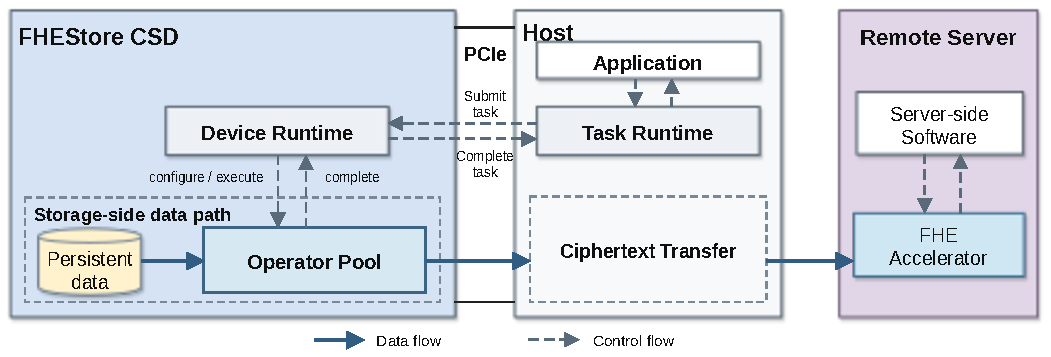
\includegraphics[width=\textwidth]{figures/fhestore-overview-v8/fhestore-overview.pdf}
  \caption{FHEStore architecture for ciphertext production. Solid blue arrows denote data flow; dashed gray arrows denote control flow.}
  \Description{Persistent data feed the CSD operator pool. The device runtime configures the pool and receives execution completion. The host application interacts with the task runtime, which submits tasks to the device runtime and receives completion notifications over PCIe. The host ciphertext transfer function retrieves generated ciphertexts from the CSD over PCIe and forwards them over the network to the remote server. The remote server contains server-side software and an FHE accelerator.}
  \label{fig:pipeline}
\end{figure*}

\subsection{Computational Storage and Application Integration}
Computational storage couples processing with storage to offload host work or reduce data movement~\cite{snia2025csmodel}. By executing operations along the storage-access path, it can process data where they are stored or accessed, instead of requiring host software to perform every transformation after a conventional read. The processing interface connects persistent data to an executable task, with task completion coordinated with the surrounding application.

Typical operations include filtering, statistical aggregation, feature selection, and decompression~\cite{ruan2019insider}. These operations combine storage access with application processing: a read can deliver selected or transformed data for the next stage of a computation. The benefit depends on the operation and its output representation. Filtering can shrink the returned data, whereas a representation-changing operation can produce a larger output.

Application integration requires abstractions for accessing data, configuring processing, and obtaining results. FPGA storage frameworks provide examples through virtual-file access, C++ interfaces with data and parameter streams, and unified HLS interfaces for memory and storage~\cite{ruan2019insider,wong2024dongle}. Such interfaces allow application code to express processing tasks and data access while the framework coordinates transfers and hardware execution. Usability therefore depends on how the system exposes task parameters, input and output locations, and completion semantics alongside the processing operators.

This combination of data access and programmable processing suits ciphertext production from persistent data. Storage access and preprocessing can feed encoding and encryption within the device. Encryption expands the representation, so operator placement determines the intermediate handoffs and buffering around ciphertext transfer. Integrating the encryption operator with storage-side streams and application control is the basis of FHEStore's architecture, presented in Section~\ref{sec:architecture}.

\section{System Overview}
\label{sec:architecture}

\subsection{System Organization}
\label{subsec:system-organization}

Figure~\ref{fig:pipeline} shows FHEStore's architecture for ciphertext production, comprising an FPGA-based computational storage device (CSD) and host software connected over PCIe. The CSD combines persistent storage, device-local buffers, and an FPGA operator pool. Its device runtime coordinates storage access and operator execution. The host task runtime translates application requests into executable work, while ciphertext transfer retrieves completed ciphertexts and delivers them to the external consumer. The remote server represents an external privacy-preserving outsourcing service equipped with an FHE accelerator.

The CSD places the encryption operator alongside the data-access and preprocessing operators. Persistent data enter device-local buffers, from which an operator graph consumes application records or values. Selection and projection can prepare the input to the encryption operator, which integrates encoding with encryption. The generated ciphertexts are collected in device-local output buffers. This placement connects encryption to the data being accessed: the production graph uses device-local input and stream handoffs between operators, while the host coordinates the task and retrieves its output.

The host and device runtimes have complementary responsibilities. The task runtime interprets the requested input, preprocessing, encryption configuration, and output destination. The device runtime binds that request to the CSD's operators and memory resources. Control messages submit the execution program and operator contexts, then report completion. Data transfers move the stored input within the CSD and carry the generated ciphertexts to the host. Ciphertext transfer uses the completed output range and its valid ciphertext length to obtain the ciphertext sequence over PCIe and forward it over the network. This division lets application control and ciphertext transfer share a task boundary while retaining distinct interfaces.

Following the producer--consumer organization in Section~\ref{sec:background}, the host and CSD belong to the data owner's trusted domain. Plaintext processing and key-dependent encryption take place within this domain. The host resolves locally held key material and supplies the LWE secret key $\mathbf{s}$ through the encryption operator's context. The task describes the requested conversion and output representation; key coefficients are supplied when preparing execution. The external consumer receives the generated ciphertexts for homomorphic computation, while local task control retains the association between their production and the source data.

\subsection{Application Task Model}
\label{subsec:application-task}

An application specifies ciphertext production through a task $T=(D,Q,E,O)$. $D$ identifies the stored input and its record schema. $Q$ specifies selection predicates and the projected field for a selective task. $E$ selects the encoding and cryptographic configuration, and $O$ identifies the ciphertext output destination. Together, these components describe which application values are to be encrypted, how they are represented, and where the resulting sequence is made available. The task runtime checks the input schema, query, and conversion configuration before submitting device execution.

The input description combines a storage range with the interpretation of its contents. For record-oriented inputs, the schema identifies record boundaries, field types, and field offsets. These properties determine how preprocessing extracts the operands needed by $Q$. Selection evaluates predicates on the source records, and projection chooses the application value passed to encryption. A task over packed application values can omit preprocessing and feed the encryption operator directly. Both forms use the same ciphertext-production interface, with preprocessing determining the values entering the encryption operator.

For a selective task over source records $r_0,\ldots,r_{N-1}$, let $\mathcal{I}_Q=(i_0,\ldots,i_{M-1})$ list the $M$ indices selected by $Q$ in source order, and let $\pi_Q$ denote its field projection. With configuration $E$ and secret key $\mathbf{s}$, the task produces
\begin{equation}
  c_j \leftarrow \operatorname{Enc}_{\mathbf{s},E}\!\left(
    \operatorname{Encode}_{E}\!\left(\pi_Q(r_{i_j})\right)
  \right),\quad 0\leq j<M.
  \label{eq:task-ciphertexts}
\end{equation}
Here, $c_j$ is the ciphertext bundle representing one projected application value under $E$. The bundle is the application-level output unit even when the encoding represents a value with multiple ciphertexts.

The task returns the ordered ciphertext sequence together with its source-record mapping $\mathcal{I}_Q$. The host derives this mapping from the selection manifest produced by device preprocessing and retains it alongside the ciphertexts. This association matters because selection changes both the number of values and their positions relative to the original records. Source order gives the consumer a consistent interpretation of sequence position, including repeated projected values from different records. An empty selection yields an empty ciphertext sequence and mapping. The output destination $O$ specifies where these task outputs become available independently of the device resources used to produce them.

\subsection{Operator Graphs and Device Execution}
\label{subsec:operator-execution}

The task runtime translates $T$ into an operator graph, operator contexts, and input and output SLM ranges. Graph nodes identify operator functions, and edges specify the streams exchanged between their ports. An execution program records the graph's operator requirements, connections, and entry and terminal endpoints for submission to the device runtime. Keeping these objects distinct connects application semantics to device execution: the graph defines the computation, contexts supply its task-specific interpretation, and SLM ranges identify the data it consumes and produces.

Operator contexts carry the record layout from $D$, selection and projection settings from $Q$, and the encryption configuration from $E$. The encryption operator's context also contains its locally supplied key material. Contexts are associated with the graph's logical operators, so each operator receives the parameters appropriate to its role. For a selective task, the operator context for preprocessing determines which fields are inspected and which field is emitted, while the operator context for encryption determines how each emitted value becomes a ciphertext bundle. Section~\ref{sec:implementation} develops the encryption operator's internal design.

An input SLM range identifies the device-local input buffer, its offset, and its byte extent. An output SLM range identifies the destination buffer and the extent available for ciphertext reception. These ranges bind graph endpoints to data locations without encoding those locations into the operator's processing logic. Their extents also distinguish the bounded input consumed by an execution from the capacity reserved for its expanded output. The device runtime receives the range bindings together with the execution program and operator contexts.

Before execution, the device runtime assigns the graph to available operators, installs their contexts, and binds stream destinations through the stream switch. The graph's logical connections determine the downstream operator or output endpoint for each stream. A selective task connects preprocessing to encryption; a task without preprocessing uses the encryption operator alone. During the production pass, preprocessing and encryption exchange values through the operator interconnect. The host therefore supplies execution control while the operator graph carries out the requested conversion over its bound input.

Completion closes the contract between execution and output access. Device completion reports the valid ciphertext length in the output SLM range after production has finished. The valid ciphertext length identifies the ciphertext sequence available for retrieval, separately from the output range's allocated capacity and execution framing. The task runtime passes the valid ciphertext length to ciphertext transfer and retains the source-record mapping. Application completion denotes availability at $O$. Section~\ref{sec:production} explains how the shared stream switch realizes these graph connections and how execution manages the expanded output.
\section{HLS Design of TFHE Encryption}
\label{sec:implementation}

FHEStore implements encoding and encryption as an HLS operator in the CSD's FPGA operator pool. The encryption operator receives application values, encodes their radix digits, and generates the ciphertext bundle consumed by the downstream application. Figure~\ref{fig:tfhe-encryption} organizes the datapath into input and context, sampling, encryption arithmetic, and packetization. These regions connect the torus-LWE operation in Section~\ref{sec:background} to the storage-side stream in Section~\ref{sec:architecture}. Encoding and encryption share the operator invocation: an application value remains in the datapath while its encoded digits become LWE blocks, and generated coefficients leave incrementally through the packetizer.

\begin{figure*}[t]
  \centering
  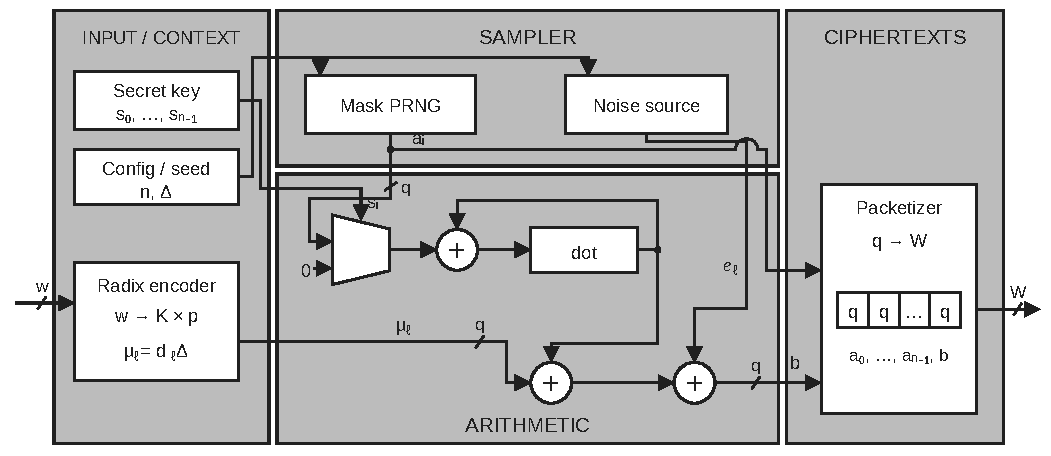
\includegraphics[width=\textwidth]{figures/tfhe-encryption-v4/tfhe-encryption.pdf}
  \caption{HLS architecture for integrated TFHE encoding and encryption.}
  \Description{Four functional regions contain input and context, mask and noise sampling, encryption arithmetic, and ciphertext packing. The radix encoder takes w-bit application values. A binary-key selector feeds a dot-product accumulator with feedback. Two additions combine the dot product, encoded digit, and noise. Mask coefficients and the body feed the packetizer, which outputs W-bit ciphertext beats.}
  \label{fig:tfhe-encryption}
\end{figure*}

\subsection{Representation and Streaming Interface}
\label{subsec:tfhe-interface}

Let $w$ denote the application-value width, $p$ the message bits per radix digit, and $K=\lceil w/p\rceil$ the number of digits representing a value. Each digit produces one LWE block with $n$ mask coefficients and a body. Thus, a ciphertext bundle contains $K$ blocks, ordered from the least-significant digit to the most-significant digit. Torus coefficients have width $q$, while the physical stream has width $W$. The packetizer places $L=W/q$ coefficients in a ciphertext beat, with $q$ dividing $W$. Widths and radix counts describe the synthesized datapath; the operator context provides the configuration for a particular execution.

The CPU coefficient layout serializes each block in natural order as $(a_0,\ldots,a_{n-1},b)$. This order gives a direct relationship between the mask index, key index, and output position. The arithmetic uses unsigned coefficients modulo $2^q$, implementing the finite-precision form of torus addition in Equation~\ref{eq:torus-lwe-encryption}. The binary secret key contains $n$ bits, with $s_i\in\{0,1\}$. Consequently, multiplication by a key coefficient becomes selection of $a_i$ or zero, followed by modular addition.

Both physical ports use AXI4-Stream. The input adapter interprets application-value framing; the packetizer constructs ciphertext beats. Configuration and the bit-packed secret key arrive through the BRAM operator context. Configuration includes the input mode, input count, and random-generator seed and nonce. Key indexing selects a context word and a bit within that word. The same key supplies successive blocks, while the coefficient index restarts at each block boundary. The encryption operator reads execution configuration before consuming its first payload beat. The input count controls application-value consumption, whereas coefficient and digit counters control block production; these counts remain separate as encryption expands each accepted value into a bundle.

The packetizer serializes each block's $n+1$ coefficients in $\lceil(n+1)/L\rceil$ ciphertext beats. Unused coefficient positions in the final beat are padding. The serialized ciphertext bundle size in bytes is therefore
\begin{equation}
  C=K\left\lceil\frac{n+1}{L}\right\rceil\frac{W}{8}.
  \label{eq:tfhe-bundle-size}
\end{equation}
Block padding belongs to this serialized representation; the terminal beat is separate.



\subsection{Integrated Encoding and Encryption}
\label{subsec:tfhe-encryption}

The input adapter supplies one application value $x$ to the radix encoder at a time. Packed mode carries consecutive values within a physical stream beat. The adapter inspects the AXI4-Stream byte-enable mask, TKEEP, and extracts the valid values in stream order. A configured input count bounds consumption when the final physical beat contains additional data. The adapter retains the received beat while its values are processed, allowing the encryption core to operate on a narrower value interface than the external stream.

Scalar mode instead assigns one application value to each payload beat, using its low $w$ bits. This framing matches a preprocessing operator that emits one projected field per selected record. Here, the beat itself identifies one value; the byte-enable mask does not specify a collection of packed inputs. Both modes present the same value interface to the encoder, so the subsequent ciphertext bundle has the same digit and coefficient order.

For a value $x$, the radix encoder extracts successive digits and maps them to integer-torus messages:
\begin{equation}
  \begin{aligned}
    d_\ell &= \left\lfloor x/2^{p\ell}\right\rfloor \bmod 2^p,\quad 0\leq\ell<K,\\
    \mu_\ell &= d_\ell\Delta.
  \end{aligned}
  \label{eq:tfhe-radix-encoding}
\end{equation}
The encoding interval $\Delta$ places each digit within the message space represented by a coefficient. With a power-of-two interval, encoding consists of a shift into the corresponding coefficient positions. In this representation, the highest digit carries the remaining high-order bits when $p$ does not divide $w$. The encoder produces each $\mu_\ell$ inside the operator, without materializing an intermediate array of encoded torus messages.

The $K$ digits reuse one encryption core sequentially. The core completes a block and its serialization before advancing to the next digit, and completes the bundle before accepting another value from the input adapter. Value and digit indices establish a ciphertext index for the mask PRNG, while the mask-coefficient index establishes the key position. This nested execution preserves the application-value order across both input modes and the least-significant-first order within each bundle.

\subsection{Coefficient Arithmetic and State}
\label{subsec:tfhe-coefficient-arithmetic}

The arithmetic core traverses a block's mask once. At each coefficient index, the mask PRNG generates $a_i$ and the key reader supplies $s_i$. The generated coefficient branches to the packetizer and the binary-key selector. The selector contributes $a_i$ when the key bit is set and zero otherwise. Starting from a zero accumulator, the feedback update is
\begin{equation}
  u_{i+1}=(u_i+s_i a_i)\bmod 2^q,\qquad u_0=0.
  \label{eq:tfhe-encryption-accumulation}
\end{equation}
After the mask traversal, the body is $(u_n+\mu_\ell+e_\ell)\bmod 2^q$. The additions shown after the accumulator in Figure~\ref{fig:tfhe-encryption} combine the dot product, encoded digit, and noise, then forward the body to the same packetizer.

The mask PRNG maintains a generator state initialized from the seed and nonce in the operator context and the ciphertext index. The noise source uses the same generator to obtain a bounded magnitude and a sign, forming $e_\ell$ after mask generation. Generator state and arithmetic state therefore follow the block's coefficient traversal.

Incremental emission removes the need to retain a complete mask vector before serialization. The datapath retains the generator state, dot-product accumulator, coefficient and digit indices, and the packetizer's partially filled beat. The packed key remains in the operator context. The accumulator's feedback is a conditional modular addition; the body additions occur after that recurrence completes. The $W$-bit output interface combines consecutive coefficients into a beat, while the arithmetic core generates those coefficients sequentially.

\subsection{Ciphertext Packetization and Completion}
\label{subsec:tfhe-packetization}

The packetizer maintains a $W$-bit register and a count of occupied coefficient positions. Each arriving mask coefficient fills the next position. A full register is emitted as a ciphertext beat, after which the register and position count reset. The body follows the mask in the same sequence and forces a flush, even when fewer than $L$ coefficient positions are occupied. Unused positions remain zero. The following LWE block starts in a fresh beat, preserving a block stride of $\lceil(n+1)/L\rceil$ beats and making block boundaries independent of input framing.

AXI4-Stream ready/valid flow control connects packetization to the surrounding data path. A blocked output write holds the pending beat and stalls progression through the coefficient traversal. The retained arithmetic and packet state preserve the relationship between generated coefficients, their accumulated contributions, and their output positions. The input adapter consequently waits while the core finishes the current ciphertext bundle. This propagation lets the shared stream switch connect encryption to upstream preprocessing and the downstream receive path using the same streaming interface.

The operator accepts a fixed input count or a stream whose length is determined by an upstream terminal beat. With a fixed count, it encrypts the requested values and waits for the terminal beat; a premature terminal beat identifies an incomplete input. The terminal beat follows all ciphertext payload and carries completion metadata separately. Payload beats remain data beats regardless of a block boundary. Separating the terminal beat from block padding lets the receive path derive the valid ciphertext length and report task completion after the ciphertext sequence has been delivered.
\section{Storage-Side Ciphertext Production}
\label{sec:production}

FHEStore connects stored inputs, preprocessing, and the encryption operator through the operator interconnect in Figure~\ref{fig:ciphertext-production}. The production path binds device-local memory to an operator graph, streams values between its operators, and collects the expanded ciphertext output. Its execution coordinates stream routing with output allocation and completion.

\subsection{Streaming Ciphertext Production}
\label{subsec:streaming-production}

Production begins by loading the task's SSD range into its input SLM range. The device runtime issues storage reads whose destination addresses point to the input SLM range. Once loading completes, the read DMA supplies its contents as an AXI4-Stream directed to the operator graph's entry. The write DMA receives the graph's final stream into an output SLM range. This organization gives storage access and operator execution a common buffered input and provides a destination for ciphertexts as encryption produces them.

Memory binding and stream routing determine different parts of this path. DMA descriptors specify the buffer addresses and byte extents accessed at the memory endpoints. Destination tags identify where a beat travels within the operator graph. An operator-to-operator handoff therefore requires a downstream destination, while the memory endpoint requires a bound range in which to read or write data. This separation lets the same operator graph execute over different bound memory ranges.

The stream switch forwards beats according to the AXI4-Stream destination field, TDEST. Figure~\ref{fig:ciphertext-production} illustrates route composition using slot and port identifiers: the upper and lower fields identify a destination slot and input port. The example route $\{3,1\}$ selects Port~1 of Operator~\#3, while the reserved terminal route $\{\mathrm{F},2\}$ selects memory-output channel~2. The scheduler binds graph edges to their destinations and configures each source operator's next-hop route. Operator controllers attach the resulting destination tag to outgoing beats. Each operator returns its output to the same stream switch, which forwards it to the next operator or the write DMA.

An operator context determines what processing occurs along these connections. For a selective task, the selection and projection operator implements $Q$ from Section~\ref{subsec:application-task}. Its operator context supplies the record layout, predicate-field offsets and types, comparison operands, Boolean expression, and projected field. The operator captures the required fields as record beats arrive and evaluates the predicate at the record boundary. Separating this processing configuration from the graph's destination bindings lets a task change the requested selection while retaining the connection between preprocessing and encryption.

During the production pass, each matching record contributes one projected value, emitted in source order. These values pass through the stream switch into the encryption operator's scalar interface described in Section~\ref{subsec:tfhe-encryption}. The encryption operator consumes each value and returns its ciphertext bundle to the switch, with the output route targeting the write DMA. Selection, projection, and encryption thus exchange intermediate application values as streams, without materializing an intermediate array in SLM. For tasks with packed application values and no preprocessing, the read DMA can supply the encryption operator directly. Both graphs retain memory bindings at the production path's input and output.

Ciphertext expansion makes flow control part of operator composition. A selected value can occupy the encryption operator while it produces multiple ciphertext beats, whereas preprocessing advances through source records and may emit values at a different rate. Operator controllers provide input FIFOs to absorb short differences in processing rate. When a downstream stage cannot accept another beat, AXI4-Stream backpressure stalls the upstream path. The same mechanism covers preprocessing, encryption, and output reception: a full downstream buffer delays further acceptance until space becomes available. This coordination keeps the connected stages within finite buffers as the stream changes from records to selected values and then ciphertext bundles.

\begin{figure}[t]
  \centering
  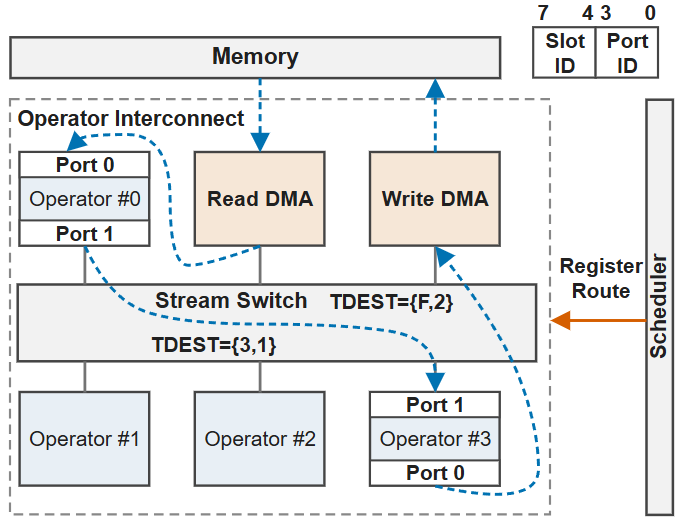
\includegraphics[width=\columnwidth]{figures/ciphertext-production-v4/author-upload.png}
  \caption{Operator interconnect and an example stream route. Dashed blue arrows show data flow.}
  \Description{Memory connects to read and write DMA endpoints above a shared stream switch. Four operator boxes surround the switch. Dashed blue arrows trace an example path from memory through read DMA, operator 0, operator 3, and write DMA back to memory. Destination labels identify the next operator port and the terminal endpoint. A scheduler beside the interconnect indicates route registration, and a field diagram shows slot and port identifiers.}
  \label{fig:ciphertext-production}
\end{figure}

\subsection{Execution and Output Management}
\label{subsec:production-management}

The output SLM range must accommodate the representation produced by the graph. Let $M$ denote the produced value count. With the serialized ciphertext bundle size $C$ defined in Equation~\ref{eq:tfhe-bundle-size}, the ciphertext payload occupies $MC$ bytes. Input bytes alone do not determine this requirement: selection determines how many values reach encryption, and encoding determines the ciphertext bundle associated with each value. The receive range reserves space for the payload and a terminal beat, rounded to the allocation alignment:
\begin{equation}
  B_{\mathrm{out}}=A\left\lceil\frac{MC+F}{A}\right\rceil,
  \label{eq:production-output-range}
\end{equation}
where $A$ is the allocation alignment and $F$ is the terminal-beat size. The valid ciphertext length is $MC$; the terminal beat and allocation padding belong to the receive extent. For tasks without selection, $M$ follows from the input value count.

For a selective task, FHEStore determines the data-dependent $M$ through a discovery pass over the input SLM range. In this mode, preprocessing produces a selection manifest with an entry for each source record, containing its index, selection flag, and selected projected value, followed by a count summary. The stream switch directs this output to the write DMA and a temporary output SLM range. Its extent is determined by the source-record count, so the selection manifest can be received before the selected count is known. The host retrieves the selection manifest and checks its record identities, selection flags, task metadata, and summary count. It then obtains $M$ and the source-record mapping $\mathcal{I}_Q$.

The task runtime uses $M$ to allocate the ciphertext output SLM range and launches the production pass with the operator graph that connects preprocessing to encryption. This pass reads the same input SLM contents and applies the same selection and projection. For $M>0$, the task uses one SSD load and two SLM scans. The discovery pass establishes the output extent and mapping; during the production pass, projected values flow directly into encryption. The selection manifest remains host-side task metadata, while the operator graph produces the ciphertext sequence. If $M=0$, the task skips the production pass and returns an empty ciphertext sequence and mapping.

Execution begins by preparing the write DMA's receive descriptors before starting the read DMA. This ordering makes the bound output range available when the operator graph starts producing ciphertexts. After the payload, the encryption operator emits a separate terminal beat. The device runtime recognizes the terminal beat in receive completion, excludes its bytes from payload accounting, and reports the valid ciphertext length. Device completion therefore identifies the point at which the graph's ciphertext output is available in SLM. Ciphertext transfer retrieves the output and uses the reported length to identify the valid sequence, including serialized block padding and excluding the terminal beat and allocation padding. The host associates the ordered ciphertext bundles with $\mathcal{I}_Q$ for selective tasks.

Larger selective tasks are divided into batches with a bounded source-record count. Each batch runs a discovery pass, sizes its output range, and executes the production pass when its selected count is nonzero. Bounding the source-record count also bounds the input buffer, selection manifest, and maximum ciphertext output extent when every record matches. Batches execute sequentially, and their device buffers are released after output retrieval. The host adjusts each batch's selected indices by its source-record offset, retaining the source-record mapping across batch boundaries. Ordered execution and source-order emission preserve the correspondence between the ciphertext sequence and its selected records as the task progresses through the stored input.

\section{Experimental Evaluation}
\label{sec:evaluation}
\subsection{Experimental Setup and Baselines}
The evaluation examines FPGA encryption performance, end-to-end ciphertext production, and interoperability with the remote server. The encryption-operator comparison measures the efficiency of FPGA TFHE encryption. The ciphertext-production comparison measures FHEStore's storage-side input path, and the ciphertext compatibility demonstration exercises homomorphic computation with its generated ciphertexts.

Table~\ref{tab:encryption-configuration} instantiates the symbolic design parameters used in Sections~\ref{sec:implementation} and~\ref{sec:production}. The mask PRNG uses a seeded xorshift generator, and the noise source produces bounded signed samples. With the CPU coefficient layout, each LWE block contains 256 mask beats followed by a beat containing the body and seven padding coefficients. The encoding interval places the two message bits at coefficient positions 60 and 59. These configuration details determine the ciphertext bundle size and output allocation used in the evaluation.

\begin{table}[t]
  \caption{Encryption and stream configuration for evaluation.}
  \label{tab:encryption-configuration}
  \centering
  \small
  \begin{tabular}{@{}p{0.61\columnwidth}p{0.28\columnwidth}@{}}
    \toprule
    Parameter & Value \\
    \midrule
    Application-value width $w$ & 8 bits \\
    Message width $p$ & 2 bits \\
    Carry / padding widths & 2 / 1 bits \\
    Radix block count $K$ & 4 \\
    LWE dimension $n$ & 2048 \\
    Coefficient precision $q$ & 64 bits \\
    Encoding interval $\Delta$ & $2^{59}$ \\
    Stream width $W$ & 512 bits \\
    Coefficients per beat $L$ & 8 \\
    Packed key context & 4 words \\
    Logical ciphertext bundle & 65,568 bytes \\
    Serialized ciphertext bundle $C$ & 65,792 bytes \\
    Allocation alignment $A$ & 4096 bytes \\
    Terminal-beat size $F$ & 64 bytes \\
    \bottomrule
  \end{tabular}
\end{table}

\begin{table}[htbp]
  \caption{Experimental platform.}
  \label{tab:implementation}
  \centering
  \small
  \begin{tabular}{p{0.47\columnwidth}p{0.36\columnwidth}}
    \toprule
    Item & Configuration \\
    \midrule
    FPGA board and device & To be supplied \\
    Storage-side execution platform & To be supplied \\
    HLS tool and version & To be supplied \\
    Achieved clock frequency & To be supplied \\
    LUT / FF / BRAM / DSP use & To be supplied \\
    Encryption configuration & Table~\ref{tab:encryption-configuration} \\
    Host CPU and software & To be supplied \\
    Storage and interconnect & To be supplied \\
    Remote server and network & To be supplied \\
    Ciphertext production boundary & To be supplied \\
    \bottomrule
  \end{tabular}
\end{table}

\writingguide{Complete Table~\ref{tab:implementation}. Specify the CPU baseline library, thread count, compiler settings, equivalent TFHE parameters and work, batch interpretation, cache state, repetitions, and summary statistic. Describe the storage input, preprocessing workload, homomorphic operation, and output destination.}

\subsection{Metrics and Measurement Boundaries}
Latency speedup is defined as
\begin{equation}
  S_b = \frac{T_{\mathrm{host},b}}{T_{\mathrm{FHEStore},b}},
  \label{eq:speedup}
\end{equation}
where $b$ identifies the measurement boundary and both latencies cover the same operation at that boundary. The encryption-operator comparison measures FPGA encryption against host CPU encryption. The end-to-end ciphertext-production comparison compares FHEStore's ciphertext production path with the host baseline. The ciphertext compatibility demonstration uses remote homomorphic computation to check the produced ciphertexts.
\writingguide{State exact start and stop points and report absolute latencies for both measured speedups. Clarify the inclusion of storage I/O, preprocessing, selection discovery where used, setup, transfers, and ciphertext transfer. Time ciphertext production through its specified ciphertext-availability point; do not sum stage times if execution overlaps.}

\subsection{TFHE Encryption and Ciphertext-Production Results}
Table~\ref{tab:results} reports encryption and ciphertext-production speedups for unsigned 8-bit application values with a 4~KiB (4096-byte) plaintext-input batch.

\begin{table}[t]
  \caption{TFHE encryption and end-to-end ciphertext-production speedups over the corresponding host baselines for unsigned 8-bit inputs with a 4~KiB plaintext batch.}
  \label{tab:results}
  \centering
  \small
  \begin{tabular}{p{0.50\columnwidth}cr}
    \toprule
    Measurement & Batch & Speedup \\
    \midrule
    FPGA encryption vs. host CPU encryption & 4~KiB & $5.33\times$ \\
    End-to-end ciphertext production vs. host baseline & 4~KiB & $3.26\times$ \\
    \bottomrule
  \end{tabular}
\end{table}

The FPGA encryption operator achieves a $5.33\times$ speedup over host CPU encryption. At the system level, FHEStore achieves a $3.26\times$ speedup in end-to-end ciphertext production over the host baseline. These results establish faster encryption and faster ciphertext production from persistent inputs in the evaluated configuration.
\writingguide{Add absolute latency and throughput results, repetitions or uncertainty estimates, and a stage breakdown. Specify whether throughput is expressed as plaintext bytes, application values, or ciphertext bytes per second.}

\subsection{Ciphertext Compatibility}
We verify ciphertext compatibility by supplying ciphertexts produced by FHEStore to the remote server for homomorphic computation.
\writingguide{Describe the demonstrated homomorphic operation, parameters, input values, and execution procedure. Compare recovered outputs with plaintext reference results. Report transfer and homomorphic computation times separately if measured.}

\subsection{Host CPU Utilization and Data Movement}
\writingguide{Measure host CPU utilization consistently across the baseline and FHEStore for ciphertext production. Report absolute utilization and define any reduction. Measure plaintext and ciphertext traffic at each relevant boundary, including selection discovery where used and the remote server connection. No utilization or traffic-reduction percentage is currently available.}

\subsection{Placement, Selectivity, and Batch Size}
\writingguide{Compare supported alternative placements, vary preprocessing selectivity where applicable, and sweep batch sizes. Measure latency, throughput, host utilization, and transfer volume. Separate FPGA acceleration from storage-side placement with an ablation where supported, and examine ciphertext output size and network transport effects.}

\subsection{Correctness and Limitations}
The performance measurements use unsigned 8-bit inputs with a 4~KiB plaintext batch and characterize TFHE encryption and ciphertext production. The ciphertext compatibility demonstration checks use of the produced ciphertexts by the external consumer.
\writingguide{Describe encryption checks, selected-count and source-order checks, and ciphertext compatibility tests. State workload and parameter coverage, trust assumptions, and conditions under which storage access, ciphertext expansion, or transport limits ciphertext production.}

\section{Related Work}
\label{sec:related}
FHEStore connects persistent data to FHE accelerators through storage-side ciphertext production. The relevant comparison axes are computation scope, data-path placement, and accelerator integration. These axes connect FHEStore to work on FHE accelerators, FPGA cryptographic engines, and computational storage.
\writingguide{Add primary-paper citations and compare input/output scope, storage-side placement, remote accelerator integration, cryptographic parameters, and measured operations. Distinguish input-encryption acceleration from homomorphic-computation acceleration, and compare speedups only at compatible measurement boundaries.}

\section{Conclusion}
\label{sec:conclusion}
FHEStore bridges persistent data and FHE accelerators through storage-side ciphertext production. The encryption operator integrates encoding with TFHE encryption, and the stream switch composes it with storage access and preprocessing. Task control binds the operator graph to operator contexts, memory ranges, and stream destinations; the host performs ciphertext transfer to the external consumer. In the evaluated configuration, the encryption operator and end-to-end ciphertext production achieve $5.33\times$ and $3.26\times$ speedups over host CPU encryption and the host baseline, respectively. The ciphertext compatibility demonstration verifies use of the produced ciphertexts by the remote server.

% Do not expose acknowledgments or identifying grant information in review.
% Add this environment, with real content, in the accepted version.
% \begin{acks}
% Acknowledge funding and assistance here.
% \end{acks}

% Start balancing in a first column, deferring if references start in a second.
\makeatletter
\if@firstcolumn
  \balance
\else
  \AddToHookNext{shipout/after}{\balance}
\fi
\makeatother
\bibliographystyle{ACM-Reference-Format}
\bibliography{FHEStore_refs}

% Optional appendix: keep only material useful for reviewing the paper.
% Check the conference's page-limit rules before adding supplementary text.
\appendix
\section{Reproducibility Details}
\label{app:reproducibility}
\writingguide{Provide commands, input data descriptions, preprocessing settings, FPGA build details, and timing procedures corresponding to the configuration in Section~\ref{sec:evaluation}. Document discovery and production passes, the homomorphic operation, ciphertext transfer, and correctness verification.}

\end{document}
